\documentclass{article}
\usepackage[utf8]{inputenc}
\usepackage[T1]{fontenc}
\usepackage[english]{babel}
\setlength{\parindent}{0pt}
\usepackage{hyperref}
\hypersetup{
    colorlinks=true,
    linkcolor=blue,
    filecolor=magenta,      
    urlcolor=cyan}
\usepackage{graphicx}
\graphicspath{ {./pic/} }
\usepackage{multicol}
\usepackage{lscape}

\usepackage{fourier,amssymb,microtype,amsmath,gensymb}
\newcommand{\R}{\mathbb{R}}
\usepackage{mdframed,caption,xcolor}
\usepackage{tikz,tkz-euclide}

\title{Seminar 4. Elasticity of Substitution}
\author{Xiaoguang Ling \\  \href{xiaoguang.ling@econ.uio.no}{xiaoguang.ling@econ.uio.no}}
\date{\today}

\begin{document}

\maketitle

%%%%%%%%%%%%%%%%%%%%%%%%%%%%%%%%%%%%%%%%%%%%%%%%%%%%%%%%%%%%%%%%%%%%%%%%%%%%%%%%%%%%%%%%%%%%%%

\begin{mdframed}[backgroundcolor=blue!20,linecolor=white]
\section{Substitution along an indifference curve}
\begin{center}
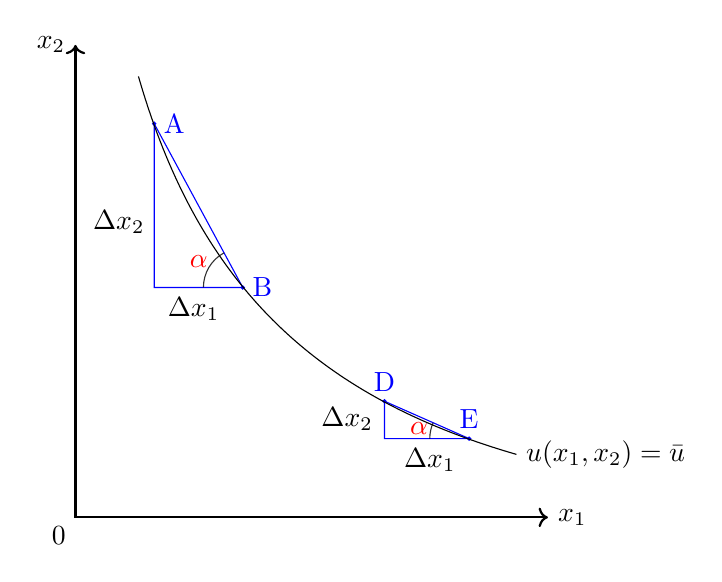
\begin{tikzpicture}[scale=0.5]

\draw[thick,<->] (0,12) node[left]{$x_2$}--(0,0)--(12,0) node[right]{$x_1$};
\node [below left] at (0,0) {$0$};

% \draw(2,9.44)--(4,5.84);
% \draw(9.44,2)--(5.84,4);

% \node[right] at (3.05,7.7) {$x^1$};
% \draw[fill] (3.05,7.56) circle [radius =0.04];
% \node[right] at (7.5,3.3) {$x^2$};
% \draw[fill] (7.56,3.05) circle [radius =0.04];

% \tkzDefPoint(2,9.44){A}
% \tkzDefPoint(4,5.84){B}
\tkzDefPoint(2,10){A}
\tkzDefPoint(4.25,5.84){B}
\tkzDefPoint(2,5.84){C}
\node[right,blue] at (A) {A} ;
\draw[fill,blue] (A) circle [radius =0.04];
\node[right,blue] at (B) {B} ;
\draw[fill,blue] (B) circle [radius =0.04];

\draw [blue] (A)--(B)--(C)--cycle;
\tkzMarkAngle[fill=yellow, opacity=0.8](A,B,C)
\tkzLabelAngle[pos= 1.3,red](A,B,C){$\alpha$}

% \draw [thick,blue] (A) -- (2,10);
% \draw [thick,blue] (B) -- (4.25,5.84);

\node[left] at (2,7.5) {$\Delta x_2$};
\node[below] at (3,5.84) {$\Delta x_1$};

% \tkzDefPoint(5.84,4){D}
% \tkzDefPoint(9.44,2){E}
\tkzDefPoint(7.85,2.95){D}
\tkzDefPoint(10,2){E}
\tkzDefPoint(7.85,2){F}
\draw [blue] (D)--(E)--(F)--cycle;
% \draw [thick,blue] (D) -- (5.84,4.25);
% \draw [thick,blue] (E) -- (10,2);
\node[above,blue] at (D) {D} ;
\draw[fill,blue] (D) circle [radius =0.04];
\node[above,blue] at (E) {E} ;
\draw[fill,blue] (E) circle [radius =0.04];

\tkzMarkAngle[fill=yellow,opacity=0.8](D,E,F)
\tkzLabelAngle[pos= 1.3,red](D,E,F){$\alpha$}

\node[left] at (7.8,2.5) {$\Delta x_2$};
\node[below] at (9,2) {$\Delta x_1$};

\draw(1.6,11.2) ..controls (3.1,6) and (6,3.1) .. (11.2,1.6) node[right]{$u(x_1,x_2)=\bar{u}$};

\end{tikzpicture}
\captionof{figure}{Marginal change and slope}
\label{fig:margin}
\end{center}
\vspace{2mm}


When we move along $u(x_1,x_2)=\bar{u}$, we can observe the following facts:
\begin{itemize}
\item The small increase of $x_1$ (i.e. $\Delta x_1$) is always followed by some small decrease of $x_2$ (i.e. $\Delta x_2$). Angle $\alpha$ reflects how much you have to give up (substitute).

\item $\alpha = - \frac{\Delta x_2}{\Delta x_1}$ depends on the relative amount of $x_1$ and $x_2$, i.e. $\frac{x_1}{x_2}$ (Note $\Delta x_2$ is negative here).
\end{itemize}

\textbf{Intuition}: To keep utility the same, you need to give up $\Delta x_2$ to consume $\Delta x_1$. 

\vspace{4mm}

\textbf{Two questions:}

\begin{itemize}
\item How to calculate $\alpha = - \frac{\Delta x_2}{\Delta x_1}$ ?
\item How to describe the relationship between $\alpha$ and $\frac{x_1}{x_2}$ ?
\end{itemize}

\section{Marginal Rate of Substitution (MRS)}

When $x_1$ increases one very small unit, we define $\angle \alpha$ as Marginal Rate of Substitution (MRS). 

$$MRS = \alpha = - \frac{\Delta x_2}{\Delta x_1}$$

We can calculate $\alpha$  in the following 2 ways:

\vspace{4mm}

\textbf{Method 1 (2-D thinking)}

Similar to Jehle \& Reny 1.27 in seminar 1, an indifference curve can be seen as the graph of a function $x_2 = f_(x_1)$ given some utility $\bar{u}$. $- \alpha$ is simply the slope (derivative), thus $\alpha = - \frac{dx_2}{dx_1}$.

An alternative way of thinking is: when line segment $A-B$ and $D-E$ are extremely short, $\alpha$ is simply the slope of the indifference curve.

\vspace{2mm}

\textbf{Method 2 (3-D thinking)}

Given $u(x_1,x_2)$ is a differentiable function (recall the hill-like 3-D graph I showed you). The small change of $u(x_1,x_2)$, i.e. $\Delta u(x_1,x_2)$, can always be attributed to the small change of $x_1$ and  $x_2$. The "attribution" of each unit change of the two commodities is called "Marginal utility", $\frac{\partial u(x_1,x_2)}{\partial x_1}$ and $\frac{\partial u(x_1,x_2)}{\partial x_2}$:

$$\Delta u(x_1,x_2) = \frac{\partial u(x_1,x_2)}{\partial x_1} \Delta x_1 + \frac{\partial u(x_1,x_2)}{\partial x_2} \Delta x_2$$

(See also \href{https://en.wikipedia.org/wiki/Total_derivative}{Total derivative}.)

Now, let's keep $u(x_1,x_2) = \bar{u}$, i.e. $\Delta u(x_1,x_2) = 0$, we have

$$0 = \frac{\partial u(x_1,x_2)}{\partial x_1} \Delta x_1 + \frac{\partial u(x_1,x_2)}{\partial x_2} \Delta x_2$$


$$ \alpha = - \frac{\Delta x_2}{\Delta x_1} = \frac{\partial u(x_1,x_2) / \partial x_1}{\partial u(x_1,x_2) / \partial x_2}$$

\textbf{Intuition:} The more important $x_1$ is, the more $x_2$ you'd like to give up.

\vspace{2mm}


Another virtue of the 3-D thinking is that it can be easily generalized to many-dimension problem. Given utility the same, \textbf{to consume more commodity $i$}, how much commodity $j$ must you give up? This is called the \textbf{Marginal Rate of Substitution of good $j$ for good $i$}:

$$MRS_{ij}(x) = \frac{\partial u(x) / \partial x_i}{\partial u(x) / \partial x_j}$$

Similarly, in the case of Production theory, given the quantity of production the same (along an isoquant), \textbf{to increase input $i$}, how much input $j$ must be decreased? This is called the \textbf{Marginal Rate of Technical Substitution of input $j$ for input $i$}:

$$MRTS_{ij}(x) = \frac{\partial f(x) / \partial x_i}{\partial f(x) / \partial x_j}$$

Here the word "Technical" refers to the technology $f(x)$.

\section{Elasticity of Substitution}

\subsection{$\alpha$ and $\frac{x_1}{x_2}$}


The relationship between $\alpha$ and $\frac{x_1}{x_2}$ also reflects the nature of the two commodities.

In Figure \ref{fig:bent} and Figure \ref{fig:flat}, the change of $\frac{x_1}{x_2}$ can be expressed by $\angle \gamma$. When $\frac{x_1}{x_2}$ changes $\gamma$:

\begin{itemize}
\item in Figure \ref{fig:bent},  the "slope" MRS changes a lot.
\item in Figure \ref{fig:flat},  the "slope" MRS changes a little.
\end{itemize}


\begin{center}
\begin{tikzpicture}[scale=0.5]
\draw[thick,<->] (0,12) node[left]{$x_2$}--(0,0)--(12,0) node[right]{$x_1$};
\node [below left] at (0,0) {$0$};
\draw(2.5,11) ..controls (3,3).. (11,2.5) node[right]{$u(x_1,x_2)=\bar{u}$};
\tkzDefPoint(0,0){O}
\tkzDefPoint(2.7,8.3){A}
\tkzDefPoint(2.7,0){B}
\tkzDefPoint(6,3){C}
\tkzDefPoint(6,0){D}
\draw [red] (O)--(A);
\draw [red] (A)--(B);
\draw [blue] (O)--(C);
\draw [blue] (C)--(D);
\node[right,red] at (A) {A} ;
\node[below,red] at (B) {B} ;
\draw[fill,red] (A) circle [radius =0.04];
\node[above,blue] at (C) {C} ;
\node[below,blue] at (D) {D} ;
\draw[fill,blue] (C) circle [radius =0.04];


\tkzMarkAngle[fill=red,size=0.8,opacity=0.4](D,O,C)
% \tkzLabelAngle[pos= 1,red](D,O,C){$\beta$}
\tkzMarkAngle[fill=blue,size=1,opacity=0.4](B,O,A)
% \tkzLabelAngle[pos= 1.5,blue](B,O,A){$\alpha$}
\tkzMarkAngle[fill=yellow,size=1.4,opacity=0.4](C,O,A)
\tkzLabelAngle[pos= 1.6,yellow](C,O,A){$\gamma$}

\end{tikzpicture}
\captionof{figure}{MRS changes much}
\label{fig:bent}
\end{center}
\vspace{2mm}


\begin{center}
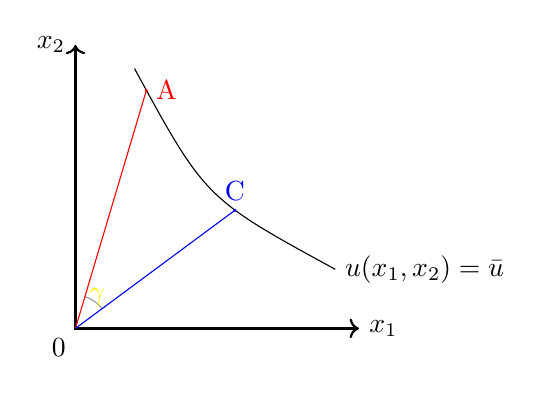
\begin{tikzpicture}[scale=0.3]
\draw[thick,<->] (0,12) node[left]{$x_2$}--(0,0)--(12,0) node[right]{$x_1$};
\node [below left] at (0,0) {$0$};
\draw(2.5,11) ..controls (5.5,5.5).. (11,2.5) node[right]{$u(x_1,x_2)=\bar{u}$};

\tkzDefPoint(0,0){O}
\tkzDefPoint(3,10.07){A}
\tkzDefPoint(6.75,5){C}
\draw [red] (O)--(A);
\draw [blue] (O)--(C);
\node[right,red] at (A) {A} ;
\draw[fill,red] (A) circle [radius =0.04];
\node[above,blue] at (C) {C} ;
\draw[fill,blue] (C) circle [radius =0.04];
\tkzMarkAngle[fill=yellow,size=1.4,opacity=0.4](C,O,A)
\tkzLabelAngle[pos= 1.6,yellow](C,O,A){$\gamma$}

\end{tikzpicture}
\captionof{figure}{MRS changes a little}
\label{fig:straight}
\end{center}
\vspace{2mm}


Now let's think about an extreme case. In Figure \ref{fig:straight}, when
$\frac{x_1}{x_2}$ changes $\gamma$, MRS does not change ($MRS_{12}(x) = \frac{\partial u(x) / \partial x_1}{\partial u(x) / \partial x_2} = 0.5$). That is, MRS is independent of $\frac{x_1}{x_2}$. 

You're never bored with $x_1$ comparing with $x_2$, no matter how much $x_1$ and $x_2$ you consumed. This can only happen when $x_1$ and $x_2$ are in nature the same commodity. 

For example, $x_1$ is an apple, while $x_2$ is a pack of 2 apples. The quality of the apples are the same and the only difference is the amount per package. Since you can always substitute a 2-apple pack with 2 single apples, we call this condition as "\textbf{perfect substitution}".



\begin{center}
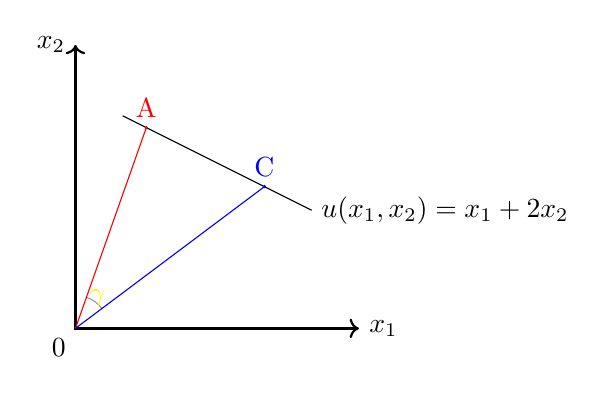
\begin{tikzpicture}[scale=0.3]
\draw[thick,<->] (0,12) node[left]{$x_2$}--(0,0)--(12,0) node[right]{$x_1$};
\node [below left] at (0,0) {$0$};
\draw(2,9) -- (10,5) node[right]{$u(x_1,x_2)= x_1 + 2x_2$};

\tkzDefPoint(0,0){O}
\tkzDefPoint(3,8.5){A}
\tkzDefPoint(8,6){C}
\draw [red] (O)--(A);
\draw [blue] (O)--(C);
\node[above,red] at (A) {A} ;
\draw[fill,red] (A) circle [radius =0.04];
\node[above,blue] at (C) {C} ;
\draw[fill,blue] (C) circle [radius =0.04];
\tkzMarkAngle[fill=yellow,size=1.4,opacity=0.4](C,O,A)
\tkzLabelAngle[pos= 1.6,yellow](C,O,A){$\gamma$}

\end{tikzpicture}
\captionof{figure}{Perfect substitution}
\label{fig:flat}
\end{center}
\vspace{2mm}

Another extreme example is Leontief preference.  In Figure \ref{fig:leo}, when $\frac{x_1}{x_2}$ changes $\gamma$, MRS changes from $+\infty$ to $0$.
We already know with Leontief preference, you believe $x_1$ and $x_2$ are totally different and can only make sense with certain proportion, like bread and cheeze. There can be \textbf{no substitution} between the two.


\begin{center}
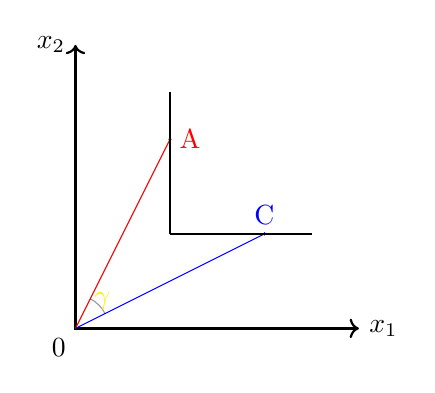
\begin{tikzpicture}[scale=0.3]
\draw[thick,<->] (0,12) node[left]{$x_2$}--(0,0)--(12,0) node[right]{$x_1$};
\node [below left] at (0,0) {$0$};

\tkzDefPoint(0,0){O}
\tkzDefPoint(4,8){A}
\tkzDefPoint(8,4){C}
\draw [red] (O)--(A);
\draw [blue] (O)--(C);
\node[right,red] at (A) {A} ;
\draw[fill,red] (A) circle [radius =0.04];
\node[above,blue] at (C) {C} ;
\draw[fill,blue] (C) circle [radius =0.04];
\tkzMarkAngle[fill=yellow,size=1.4,opacity=0.4](C,O,A)
\tkzLabelAngle[pos= 1.6,yellow](C,O,A){$\gamma$}

\draw [thick] (4,10) -- (4,4);
\draw [thick] (4,4) -- (10,4);

\end{tikzpicture}
\captionof{figure}{Leontief Preference}
\label{fig:leo}
\end{center}


\section{Elasticity of Substitution $\sigma_{12}$}

We can use "\textbf{Elasticity}" to reflect the relationship between $\alpha$ and $\frac{x_1}{x_2}$.

$Elasticity = \frac{\Delta MRS /MRS}{d}$


DEFINITION: The Elasticity of Substitution (a 2-input case for DEFINITION 3.2 on Jehle \& Reny pp. 129)

\vspace{2mm}

For a production function $f(x_1,x_2)$, the elasticity of substitution of input $2$ for input $1$ at the
point $(x_1,x_2) \in \R^2_{++}$ is defined as:

$$\sigma_{12}(x_1,x_2) \equiv (\frac{d ln MRTS_{12}(\frac{x_2}{x_1})}{dln (\frac{x_2}{x_1})})^{-1}$$

Note both the numerator and the denominator are functions of $\frac{x_2}{x_1}$. If we define $\frac{x_2}{x_1} = r$,
$\sigma_{12}(x_1,x_2)$ can be rewritten as:

$$\sigma_{12}(x_1,x_2) \equiv (\frac{d ln MRTS_{12}(r)}{dln r})^{-1}$$






\textbf{An example from exam 2019 Q1(b)}

Deb and Frank have the following utility functions


\end{mdframed}






\end{document}
